\chapter{The Information Framework} \label{chap_InformationFramework}

%citazione introduttiva
\epigraph{\textit{Pure mathematics is, in its way, the poetry of logical ideas.}}{Albert Einstein}


Supply chains systems involve a large number of connected entities, resources, actors and flows.  In this chapter, we introduce a framework to model the entities of storage systems, distribution networks and production plants. In particular, this work investigates the room for the application of data science in the field of logistics and operations. For this reason, we are interested in mapping the information relationships between these entities.\par

Here we introduce an ontology of entities and metrics. This ontology meets the \textit{fractal manufacturing system} philosophy (see \cite{Sprock2018}), where each element of a supply chain can be seen as a black box with inputs and outputs. The elements can be aggregated or disaggregated into other black boxes. In the following parts of this book, we will re-define this ontology by applying it to smaller blocks of the supply chain, with specific references to storage systems, distribution networks and production plants.

\section{Ontology}\label{secOntology}
We base our ontology on \cite{Hopp2011}, a milestone book in logistics and operations science. It was the first providing a scientific framework to model a factory. 

\subsubsection{Entities}
We identify the following entities.\par
\textbf{Part} ($i$): it is a piece of raw material, component, subassembly or assembly. Where:
\begin{itemize}
    \item Raw material is a part purchased out of the system.
    \item Component is an individual piece assembled into more complex products.
    \item Subassembly is an assembled unit further assembled into more complex products.
    \item Assembly/final assembly/finished product is the fully assembled product.
\end{itemize}
\par
\textbf{Processing node} ($j$): we define the processing node using the concept of fractal manufacturing. From this perspective, a processing node is any entity that can be modelled as a black box with input and output. A production machine, a production line, a packing machine, a manufacturing robot, a production plant, a storage system, a port, a logistic platform, a train terminal are all examples of entities working as a processing node. A processing node usually performs value-added activities on a part. \par

\textbf{Edge} ($j,k$): it is a physical connection between processing nodes. Aisles and conveyors are edges in a production plant; while railways, rivers and roads are the edges of a distribution system.\par

\textbf{Vehicle} ($v$): a vehicle is a handling unit able to transport one or more parts from a processing node to another. Operators, forklifts, AGVs, trucks, trains, vessels are all examples of a vehicle. \par

\textbf{Consumable} ($s$): a consumable is a material that is used by a processing node or a vehicle to perform its work. A consumable is generally responsible for the variable costs of the processing node or a vehicle (e.g. energy and fuel).\par

\textbf{Route} ($e$): is the sequence (ordered set) of processing nodes $j=1,\ldots,m$ visited by a vehicle to add value on a part.\par

\textbf{Order} ($o$): is a processing request on a part sent by a customer. \par

\textbf{Job} ($b$): is the response to the market demand from the operations side. Production batches and transportation loads are examples of a job.\par

\textbf{System network} $G(V,A)$: the system network is the set of processing nodes $j\in V$ and edges $\left(j,k\right)\in A$ that connect all the entities involved in the supply chain system.

\subsubsection{Metrics}
We identify the following metrics to assess the performances of a processing node $j$.\par

\textbf{Throughput} ($TH_{j}$): the throughput of a processing node is the average output per unit of time (e.g., parts per hour).\par

\textbf{Work in process} ($WIP_{j}$): is the number of parts (i.e., the level of inventory) being processed/waiting for processing by a processing node.\par

\textbf{Work in process} ($WIP_{jk}$): is the number of parts (i.e. the inventory position) being transported on edge $(j,k)$ by a vehicle $v$. \par

\textbf{Capacity} ($C_j$): is the upper bound of the throughput.\par

\textbf{Capacity} ($C_v$): is the maximum capacity of a vehicle $v$. \par

\textbf{Utilisation} ($U_j$): it is the fraction of time that a processing node is not idle for lack of demand. \par

\textbf{Utilisation} ($U_v$): is the fraction of transportation space that a vehicle uses due to the variability of the transportation demand. \par

\textbf{Lead time} ($LT_e$): is the time allocated for a given route. \par

\textbf{Cycle time} ($CT_e$): is the average time from the release of a job to the end of its route. \par

\textbf{Service level} ($SL_e$): $Prob\{cycle\ time\le lead\ time\}$

Little’s law (see equation (\ref{eq_littlesLaw})) defines a basic relationship linking the three main metrics, i.e. $WIP$, $TH$ and $CT$.

\begin{equation}
WIP_j [pz]=TH_j \left[\frac{pz}{h}\right] \times CT_{e:e \in \{j\} } [h]
\label{eq_littlesLaw}
\end{equation}

Usually, managers have data on the entities at their disposal, but they need to get information on the metrics. This data can be dirty or incomplete. For this reason, we build upon this ontology to show how to infer the properties of entities and metrics when data are incomplete or missing.\par

Our approach is highly generalisable and based on a few standard rules of a supply chain, with minimum bias. For this reason, the theoretical effort of this work stands in the definition of a structure for industrial data, the understanding of the role of data, and the consistency rules among different features that can be used to increase the value of an incomplete dataset.\par

The modelling of a system accordingly with a robust data structure allows using only logistics-relevant data and base the model on robust relationships. The following sections define this data structure for storage, distribution and production systems. We first introduce the law of physics to analyse the material flows of a supply chain. Then, a theorem regulating the consistency of the information flow is introduced and demonstrated.\par


\section{The physics of a supply chain} \label{sect_supplyChainPhysics}

The laws of physics can be used to model the material flows between the entities of a supply chain. We can think of a processing node $j$ as a physical system with an inventory $WIP_j$ subjected to “forces” modifying its value. It is not difficult to imagine that the value of $WIP_j$ can change when:
\begin{itemize}
    \item some forces \textit{pull} a number of items from $j$;
    \item 	some forces \textit{push} a number of items into $j$.
\end{itemize}

% INSERT fig_processingNode
\begin{figure}[hbt!]
\centering
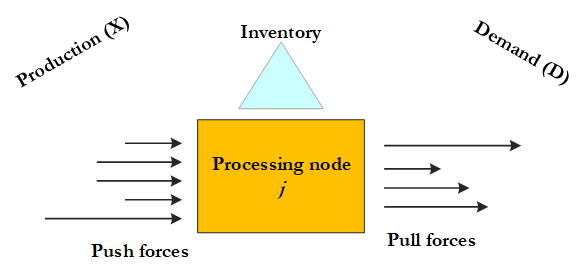
\includegraphics[width=1\textwidth]{SectionIntroduction/informationFramework_figures/fig_processingNode.png}
\captionsetup{type=figure}
\caption{Physical model of a processing node.}
\label{fig_processingNode}
\end{figure}

Figure \ref{fig_processingNode} presents a scheme of the physical model of a processing node where the forces generated by the production and the demand modify the value of the inventory.\par

The concept of a \textit{force} modifying the inventory matches very well with the definition of pull and push production philosophy. The analysis of push and pull systems is out of the scope of this book. We will limit to describe the dynamics and the rules of these systems using the idea of a \textit{force} associated with the production and the demand. To model $j$, we are just interested in defining how these forces are linked to the value of $WIP_j$. \par

The purpose of a supply chain is to provide a physical connection between demand and offer. A supply chain connects several processing nodes to develop a product or a service to the final consumer. Processing nodes works at a variable rate, and the only way to keep them synchronised is by using buffers. There are three types of buffers with different nature:
\begin{itemize}
    \item \textbf{inventory buffer} is a number of goods stored between the production and the demand of a processing node;
    \item \textbf{time buffer} is an amount of queuing time between the time instant when the order of a customer occurred and the time instant when it is finally satisfied;
    \item \textbf{capacity buffer} is an amount of production capacity calculated as the difference between the capacity of a working station and its average demand.
\end{itemize}

These types of buffers are interrelated and react to the demand and production forces. Time and capacity buffers are generally defined in the design phase of a network since they are linked with the type of physical assets of the supply chain. Inventory buffers are generally more flexible and more used since they are cheaper than the two others. \par

We use an approach based on dynamic and stochastic system equations to generalise the Little’s law, and understand the relationships between the variables describing the physics of a supply chain.\par

We can model a production-inventory model as follows. Let consider the inventory of a processing node measured in a number of parts. We are interested in knowing the value of the inventory function $q$. The inventory function depends on the demand function $d$, and the production function $x$. Figure \ref{fig_demandProduction} identifies samples demand and production functions.\footnote{The source code of Figure \ref{fig_demandProduction} is available \href{https://github.com/aletuf93/logproj/blob/master/examples/Supply\%20chain\%20physics.ipynb}{here}.} The demand curve is generally more volatile, while the production curve is more stable since the output of a processing node is hardly flexible as related to its assets.

% INSERT fig_demandProduction
\begin{figure}[hbt!]
\centering
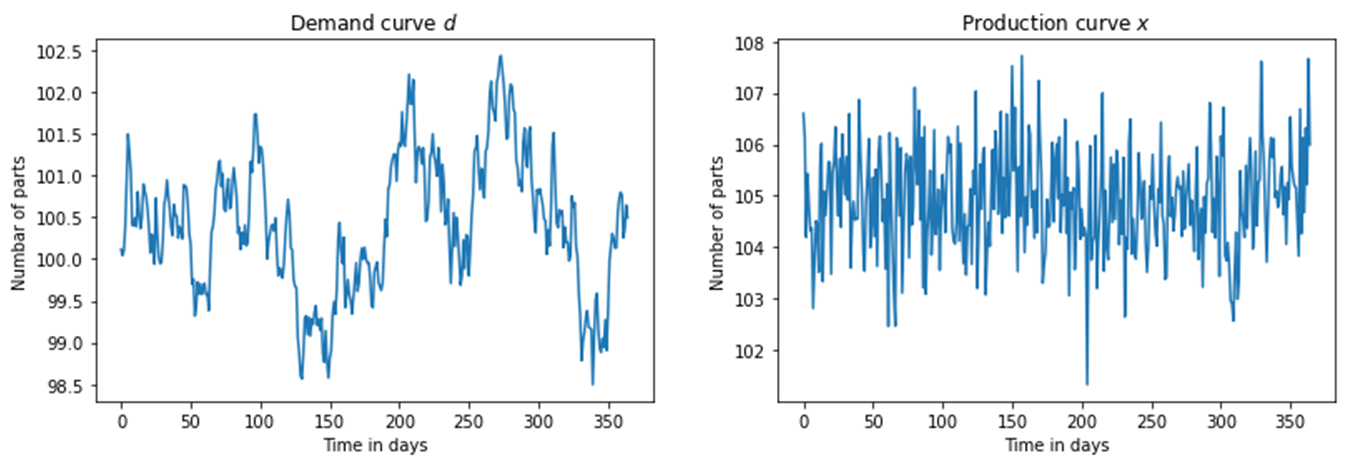
\includegraphics[width=1\textwidth]{SectionIntroduction/informationFramework_figures/fig_demandProduction.png}
\captionsetup{type=figure}
\caption{Examples of demand and production functions.}
\label{fig_demandProduction}
\end{figure}

Given $x$, $d$, and an initial inventory $q_0$, it is possible to define the inventory function $q$.

\begin{equation}
q_t=\ q_{t-1}\ +\ p_t\ -\ d_t\ 
\label{eq_physics1}
\end{equation}

The difference between the demand and production functions define the \textit{momentum} $p$ of the production node. The momentum indicates the direction in which the inventory function $q$ moves, and it is measured as the number of parts per unit of time.

\begin{equation}
p=x-d=\dot{q}
\label{eq_physics2}
\end{equation}

We identified an approach to model a supply chain using the law of physics. In particular, there is a relationship between the flows (demand $d$ and production $p$) and the inventory $q$. We can assume that some forces (may them be "push" or "pull" forces) play a role in changing the value of the inventory function $q$. Table \ref{tab_classicalMechanics} illustrates the parallelism between classical mechanics and the physics of a supply chain.

% INSERT tab_classicalMechanics
\begin{figure}[hbt!]
\centering
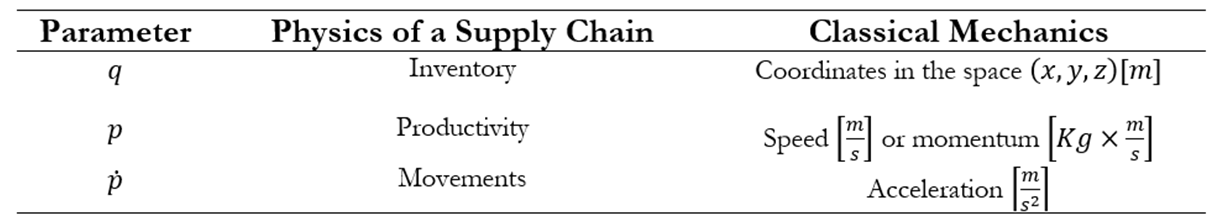
\includegraphics[width=1\textwidth]{SectionIntroduction/informationFramework_figures/tab_classicalMechanics.png}
\captionsetup{type=figure}
\caption{Examples of demand and production functions.}
\label{tab_classicalMechanics}
\end{figure}

\cite{Spearman2014} demonstrated that the energy conservation law is appliable to the physics of a supply chain to control the behaviour of the inventory curve $q$ The Lagrangian is used to express the equation of the force $\dot{p}$, representing the "push" and "pull" forces of a supply chain, i.e. the movements of the supply chain.

\begin{equation}
\dot{p}=\frac{\partial L(q,\dot{q})}{\partial q}
\label{eq_physics3}
\end{equation}

Where $L\left(q,\dot{q}\right)=\frac{1}{2}p^2-V(q)$. The Lagrangian express a difference between kinetic and potential energy. The potential energy is defined using a linear potential $V\left(q\right)=-F_0q$. This means that, as it works with the force of gravity, the perturbation of the value of the inventory depends on the value of the inventory $q$ with a linear law. We can assume conservation of energy using the Hamiltonian principle (the Principle of Least Action). This principle states that nature always chooses the lowest energy path (i.e. the difference between kinetic and potential energy) between all the feasible ones defined by forces. The inventory function $q$, is then, defined from the Lagrangian as:

\begin{equation}
S\left[q\right]=\int_{t_1}^{t_2}{\ L(q,\dot{q},t)dt}=0
\label{eq_physics4}
\end{equation}

\cite{Spearman2014} shows how choosing the value of $F_0$ to control the value of inventory $q$.


\section{The information of a supply chain}
Section \ref{sect_supplyChainPhysics} demonstrated that a physical relation exists between three variables of a supply chain: the inventory $q$, the productivity $p$, and the movements $\dot{p}$. Physics is the core of science, and we can always rely on physical laws. Nevertheless, in practice, we may not have the possibility to apply these laws since data are collected with different granularities (i.e. referred to different processing nodes) or with inconsistencies. For this reason, this section introduces an original information framework to build $q$, $p$, and $\dot{p}$ using the available data. We move the focus from the physical relationship to the information relationship existing between these three functions.

\subsection{Information framework} \label{secInfoFramework}
While defining data structures to support logistics, databases are usually designed using an entity-relationship (ER) model ~\cite{Lake2013}. The focus of ER models is on the entities, i.e. the ones we defined in section \ref{secOntology}. Here we propose a different perspective, focusing on the physical logistic phenomenon, i.e. the variation in the demand $d$, production $x$ and inventory $q$ due to the forces $\dot{p}$, regardless of the entities generating these forces.\par

This change of perspective enhances the flexibility of this modelling approach since it is often difficult to collect data from all the entities involved in a supply chain and to connect them into an ER model. On the other side, the effect of the forces generated by these entities is clearly measurable on the production and demand functions.

For the sake of clarity, we abandon the dot notation, and we define:
\begin{enumerate}
    \item a movement function $M_i(t)$ to represent the forces $\dot{p}$, applied to a part $i$;
    \item a productivity function  $P_j(t)$ to represent the speed $p$ at which the forces change the value of the inventory $q$;
    \item an inventory function $I_i\left(t\right)$ representing the inventory $q$ of part $i$.
\end{enumerate}

The $M$ function has different granularity (e.g. order, vehicle, terminal, network) depending on the measurement system and the data collection system used. The most granular is a movement called by a single order $o$ of a part $i$ involving a processing node $j$ and a vehicle $v$. The function uses:

\begin{itemize}
    \item a positive value to describe the physical movement of a quantity $q$ from a processing node to a vehicle (load movement: $j\rightarrow v$);
    \item a negative value to describe a physical movement of a quantity $q$ from a vehicle to a processing node (offload movement: $v\rightarrow j$).
\end{itemize}


\begin{equation}
M_o^{j,v}(t) =\left\{
                \begin{array}{ll}
                 q & if \  t=t_{IN}, \\
                -q & if \  t=t_{OUT}, \\
                0 & otherwise.
                \end{array}
              \right.
\label{eq_movements}
\end{equation}

Where $t$ measures the time; $q$ is the quantity (e.g. the number of parts) involved in the physical movement; $t_{IN}$ is the timestamp when the part $i$ is loaded on a vehicle $v$; $t_{OUT}$ is the timestamp when it is unloaded from it.\par

The inventory function $I$ describes the inventory position (e.g. the number of parts) of a vehicle $v$ or a processing node $j$. The function $I$ is linked to $M_o^{j,v}(t)$ by aggregating the movements of single orders.\par

\begin{equation}
I_j(t) = I_j(t-\epsilon) -\sum_{i}\sum_{v}M_o^{j,v}(t) 
\label{eqInvj}
\end{equation}

\begin{equation}
I_v(t) = I_v(t-\epsilon) +\sum_{i}\sum_{j}M_o^{j,v}(t) 
\label{eqInvv}
\end{equation}

The parameter $\epsilon$ is a sufficiently small time sampling unit (e.g. a minute). It is essential to consider the initial inventory $I_j(t=0)$ and $I_v(t=0)$ to define the inventory functions correctly. Figure \ref{fig_movementsInventory} represents an example of the movements and inventory functions for a part $i$. 

% INSERT fig_movementsInventory
\begin{figure}[hbt!]
\centering
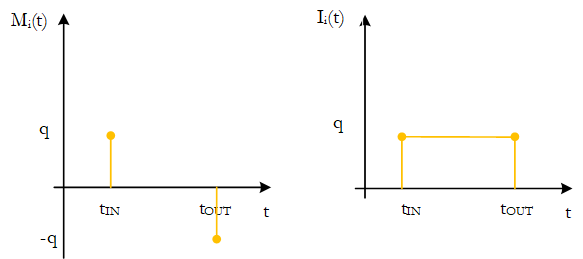
\includegraphics[width=1\textwidth]{SectionIntroduction/informationFramework_figures/fig_movementsInventory.png}
\captionsetup{type=figure}
\caption{Example of movements and inventory function.}
\label{fig_movementsInventory}
\end{figure}

The productivity function $P$ defines the motion equation of a processing node $j$, i.e. the speed of the changes in its inventory position. Two distinct $P$ functions exist to describe the loads (IN), and the offloads (OUT) speed of a processing node. The productivity function $P$ is defined, starting from the cumulative function of the movements $Q$.

\begin{equation}
Q_j^{IN}(\tau)=\sum_{i}\sum_{v}\{M_i^{j,v}|M_o^{j,v}>0,t\leq \tau \}
\label{eqQIN}
\end{equation}

\begin{equation}
Q_j^{OUT}(\tau)=\sum_{i}\sum_{v}\{M_i^{j,v}|M_o^{j,v}<0,t\leq \tau \}
\label{eqQOUT}
\end{equation}

The productivity $P$ at a time instant $t^\ast$ is given by:

\begin{equation}
P_j^{IN} (t^* )=\frac{dQ_j^{IN} (\tau)}{d\tau}\vert_{t^*}
\label{eqProdIN}
\end{equation}

\begin{equation}
P_j^{OUT} (t^* )=\frac{dQ_j^{OUT} (\tau)}{d\tau}\vert_{t^*}
\label{eqProdOUT}
\end{equation}

Movements usually have redundant information on vehicles ad processing nodes. We overcome this redundancy by splitting this information into two separate functions of inventory $I$ and productivity $P$. Productivity function, in fact, does not suffer redundancies, and it converges to a value determined by the physical assets of a terminal. \par

At this stage, we want to demonstrate the relationship between these three functions. For this reason, we consider the movement function at the granularity of a processing node $M_j(t)=\sum_{v}\sum_{o}{M_o^{j,v}(t)}$  and we prove the following theorem that introduces consistency rules between the functions $M_j$, $I_j$ and $P_j$ calculated with the granularity of a processing node $j$. \par

Let us consider the supply chain system as a network $G(V,A)$ where $V$ is the set of the processing nodes connected by arcs $(j,k)\in A$. Let us define a set $B$ containing the vehicles $v\in B$, travelling on the arcs $(j,k)\in A$. We define a state function $\Lambda(\tau)$ to describe the state of the network $G$ at the time instant $\tau$.   


\begin{equation}
\Lambda\left(\tau\right)=\ \left\{I_j\left(\tau\right),\ j\in V\ \bigcup{I_v\left(\tau\right),v\in}B\right\}
\label{eq_stateLambda}
\end{equation}

We demonstrate that:

\begin{theorem} \label{theor_MIP}
One of the following set of equations 
\begin{enumerate}[label=(\roman*)]
    \item $M_j(t)$
    \item $I_j(t)$
    \item $P_j^{IN} \bigcup P_j^{OUT} $
\end{enumerate}
has enough information to define the state $\Lambda$ of a logistic network. 
\end{theorem}

\begin{proof}

We demonstrate Theorem 1 by showing that the knowledge of (i), (ii), or (iii) is enough to define all the three $M$, $I$, and $P$. Statement (i) has already been demonstrated by the \ref{eqInvj}, \ref{eqProdIN} and \ref{eqProdOUT}. Statement (ii) can be proved considering the definition of $I$, since:


\begin{equation}
M_j(t)=I_j(t)-I(t-\epsilon) 
\label{eqThPart2}
\end{equation}

Given $M_j (t)$ the functions $P_j^{IN}$ and $P_j^{OUT}$ are calculated similarly to \ref{eqProdIN} and \ref{eqProdOUT}. \par
Statement (iii) can be proved considering:

\begin{equation}
Q_j^{IN} (\tau)=\int_0^\tau P_j^{IN}(t)dt
\label{eqThPart3IN}
\end{equation}

\begin{equation}
Q_j^{OUT} (\tau)=\int_0^\tau P_j^{OUT}(t)dt
\label{eqThPart3OUT}
\end{equation}

By sampling the functions $Q$ with a sampling frequency $\epsilon$ (e.g. a minute), it is possible to get the movement function.

\begin{equation}
M_j(t)=\frac{dQ_j^{IN}(t)}{dt} - \frac{dQ_j^{OUT}(t)}{dt}
\label{eqThPart3Mov}
\end{equation}

\end{proof}

The proof of Theorem \ref{theor_MIP} shows that the functions $M$, $I$ and $P$ are interconnected, and retain enough information to define the state $\Lambda$ of the network when they are measured with terminal granularity. 

\subsection{Implementation and utilisation of the framework}
The following chapters of this work start from the application of this information framework to warehouses, production and distribution system. The consistency rules between the metrics of movements, inventory and productivity, are the starting point to collect, store and analyse data leading, and to generate knowledge from this data.\par

We start with the definition of a data structure able to host movements and inventory data of a specific type of processing node. Then data-driven methodologies are proposed to build prediction models addressing node-specific problems. ER structures are designed to store both planning or actual data. In particular:

\begin{itemize}
    \item planning data, (i.e., recorded before it happens what they describe) describes how operations are planned to be performed;
    \item actual data (i.e., recorded when it happens what they describe), describes how activities were performed.
\end{itemize}

Table \ref{tab_MIPinLS} qualitatively introduces different types of data recorded on-field and used in the following sections to populate the data structure, according to the $M, I, P$ framework.

% INSERT tab_MIPinLS
\begin{figure}[hbt!]
\centering
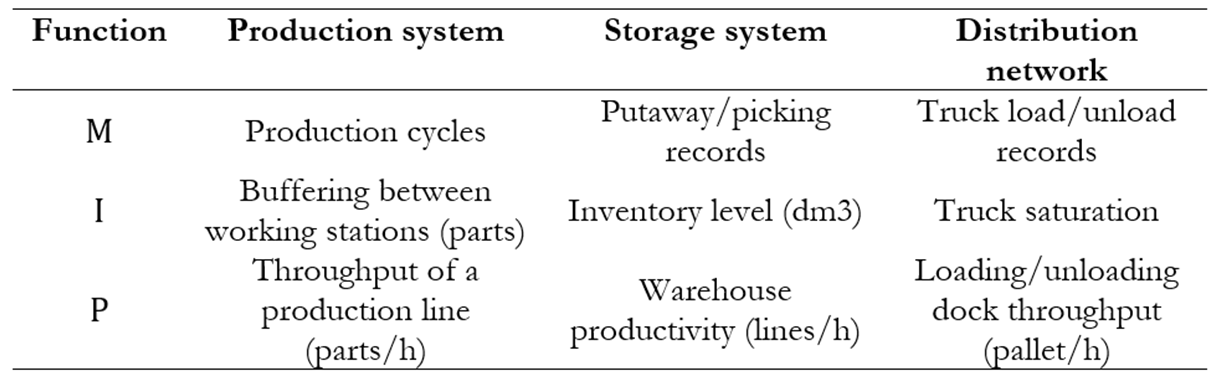
\includegraphics[width=1\textwidth]{SectionIntroduction/informationFramework_figures/tab_MIPinLS.png}
\captionsetup{type=table}
\caption{Examples of datasets connected to the functions.}
\label{tab_MIPinLS}
\end{figure}

\clearpage


%\clearpage
\bibliographystyle{ieeetr}
\bibliography{SectionIntroduction/informationFramework_ref}